\documentclass[french]{beamer}
\usepackage[utf8]{inputenc}
\usepackage[T1]{fontenc}
\usepackage{graphicx}
\usepackage{caption}
\usepackage{babel}
\usepackage{dsfont}
% This is the file main.tex

\usetheme{Berlin}
\title{Modélisation et détection de délit d'initié \\ Soutenance mi-parcours P3A}
\author{Heang Kitiyavirayuth, Lucas Broux}
\date{\today}

% Create a frame at the beginning of a section.
\AtBeginSection[]{
  \begin{frame}
  \vfill
  \centering
  \begin{beamercolorbox}[sep=8pt,center,shadow=true,rounded=true]{title}
    \usebeamerfont{title}\insertsectionhead\par%
  \end{beamercolorbox}
  \vfill
  \end{frame}
}

% Document.
\begin{document}

\begin{frame}
\titlepage
\end{frame}

\section*{Outline}
\begin{frame}
\tableofcontents
\end{frame}


\section{Introduction}
\subsection{Sujet choisi, problématique générale}
\begin{frame}
  \begin{itemize}[<+->]
    \item \textbf{Modélisation et détection de délit d'initié.}
    \item Problématique concrète mais actuellement assez mal résolue.
\end{itemize}
\frametitle{Sujet choisi}
\end{frame}

\subsection{Objectifs du projet}
\begin{frame}
  \begin{itemize}[<+->]
    \item Comprendre et analyser des articles sur le sujet :
    \begin{itemize}
%    \item [1] A. Grorud, M. Pontier, Comment détecter le délit d'initié, C.R. Acad. Sci. Paris, t. 324, p. 1137-1142, 1997.
	\item [1] A. Grorud, M. Pontier, Insider trading in a continuous time market model, International Journal of Theoretical and Applied Finance, 1, p. 331-347, 1998.
	\item [2] H. Föllmer, P. Imkeller, Anticipation cancelled by a Girsanov transformation: a paradox on Wiener space, Ann. Inst. H. Poincaré Probab. Statist 29.4, 569-586, 1993.
	\end{itemize}
    \item Pour la suite du projet ? A préciser...
\end{itemize}
\frametitle{Objectifs du projet}
\end{frame}

\section{Compréhension actuelle du problème}
\subsection{Modélisation mathématique}
\begin{frame}
\frametitle{Modèle de marché financier}
On considère un modèle de marché financier sur l'espace de probabilité $(\Omega, (\mathcal{F}_t, t \in [0,T]), \mathbb{P})$. Les prix des actions (ici $d$ actions) évoluent selon l'équation différentielle stochastique linéaire : 
\begin{center}
$\displaystyle S^i_t = S^i_0 + \int_{0}^{t} S^i_s b^i_s ds +  \int_{0}^{t} S^i_s \sigma^i_s dW_s,$\
$0 \leq t \leq T, S_0 \in \mathbb{R}^d, i = 1, ... , d$
\end{center}
\end{frame}
\newpage

\begin{frame}
\frametitle{Modèle de marché financier}
où : 
\begin{itemize}
\item $W$ est un mouvement brownien de $d$-dimension.
\item Les paramètres $b, \sigma$ et $r$ sont dans $\mathbb{R}^d, \mathbb{R}^{d\times d}, \mathbb{R}$ respectivement et sont supposés bornés sur $[0,T]$ et $\mathcal{F}$-adaptés.
\item La matrice $\sigma_t$ est inversible.
\item $S^0$ évolue d'après l'équation $S^0_t = 1 +\int_{0}^{t}S^0_s r_s ds$.
\end{itemize}
\

\textbf{H1} : La matrice $\sigma$ est inversible, $dt \otimes d\mathbb{P}$ -presque sûrement, $\eta_t = \sigma^{-1}_t (b_t - r_t \textbf{1})$ vérifie $\exists A \in ]0, T[, \exists C, \exists k > 0, \forall s \in [0, A]$, $\mathbb{E}_{\mathbb{P}}[exp(k||\eta_s||^2)] \leq C$.\
\end{frame}

\begin{frame}
\frametitle{Informations sur l'initié}
Un des investisseurs sur le marché connait l'information $\mathcal{F}_t$ qui est l'information normalement disponible au temps $t$, et il connait aussi une variable aléatoire $L \in L^1(\mathcal{F}_T)$. L'information totale dont il dispose est donc $\mathcal{F}_t \vee \sigma(L)$ (que l'on note $\mathcal{Y}_t$), qui est à priori plus grande que $\mathcal{F}_t$.\\
\

Avec cette information $\mathcal{Y}_t$, l'initié cherche à optimiser sa stratégie de consommation et de placement sur le marché.
\end{frame}

\begin{frame}
\frametitle{Informations sur l'initié}
\begin{itemize}
\item L'initié dispose d'un capital $X_0$ à l'instant $t=0$.
\item Il consomme à une vitesse $c$ qui est un processus positif et $\mathcal{Y}$-adapté, vérifiant $\int_{0}^{T} c_sds < \infty$ p.s. 
\item Il place sur l'actif $i$ la quantite $\theta^i$ et on note $\pi^i_t = \theta^i_t S^i_t$ la somme investie sur la $i$-ième action pour $i = 1,...,d$.
\item Sa richesse au temps $t$ s'exprime donc par :
\begin{center}
$X_t = \sum_{i=0}^{d} \theta^i_t S^i_t - \int_{0}^{t} c_s ds$.
\end{center}
\end{itemize}
\end{frame}

\begin{frame}
\frametitle{Informations sur l'initié}
\begin{itemize}
\item Son portefeuille est considéré autofinançant, c'est-à-dire : 
\begin{center}
\textbf{H2} : $dX_t = \sum_{i=0}^{d}\theta^i_t dS^i_t - c_t dt$.
\end{center}
\item En notant $R_t = (S^0_t)^{-1}$ le facteur d'actualisation, sous la probabilité $\mathbb{P}$, la richesse $X$ actualisée vérifie l'équation : 
\begin{center}
$X_t R_t + \int_{0}^{t} R_s c_s ds = X_0 +  \int_{0}^{t} \langle R_s\pi_s, b_s - r_s \textbf{1} \rangle ds + \int_{0}^{t} \langle R_s \pi_s, \sigma_s dW_s \rangle$
\end{center}
\end{itemize}
\end{frame}

\begin{frame}
\frametitle{Méthode du grossissement de la filtration brownienne}
\textbf{HC} : $L \in \mathbb{D}^{2,1}$ est tel que $\int_{t}^{T} ||D_u L||^2 du >0, \mathbb{P}-p.s. \forall t \in [0,T[$,\\
ou $D$ est le gradient stochastique usuel associé à W et $\mathbb{D}^{p,q}$ est l'espace de Sobolev construit à l'aide de $D$.\\
\

Sous \textbf{HC}, on a : 
\begin{itemize}
\item La loi conditionnelle de $L$ sachant $\mathcal{F}_t$ est absolument continue et il existe une version mesurable de la densité conditionnelle $(\omega, t, x) \longmapsto p(\omega, t, x) = p(0,x) + \int_{0}^{t} \alpha(\omega, t, x)dW_s$, qui est une $(\mathcal{F}, \mathbb{P})$-martingale.
\end{itemize}
\end{frame}

\begin{frame}
\frametitle{Méthode du grossissement de la filtration brownienne}
\begin{itemize}
\item Si $M = M_0 + \int_{0}^{t} \beta_s dW_s$ est une $(\mathcal{F}, \mathbb{P})$-martingale locale continue, alors le crochet $d\langle M,P \rangle_t = \langle \alpha, \beta \rangle_tdt$ et le processus $\tilde{M_t} = M_t - \int_{0}^{t}\frac{\langle \alpha(.,x),\beta\rangle_{u|x=L}}{p(u,L)}du$ est une $(\mathcal{Y}, \mathbb{P})$-martingale locale.
\item En corollaire, on obtient que le processus vectoriel $(B_t = W_t - \int_{0}^{t} l_udu, t \in [0,T[)$ est un mouvement brownien sur l'espace de probabilité filtré $(\Omega, (\mathcal{Y}_t , t \in [0, T[), \mathbb{P})$, où $l_u = \frac{\alpha(u,L)}{p(u,L)}$. 
\end{itemize}
\end{frame}

\begin{frame}
\frametitle{Changement de probabilité}
On effectue un changement de probabiliteé pour se ramener à une mesure neutre au risque.
\begin{itemize}
\item Pour ce faire, il faut définir $\xi_t = - l_t - \eta_t $.\\
\end{itemize}
\textbf{HN} : $\mathbb{E}_\mathbb{P} [exp\frac{1}{2} \int_{0}^{A} ||\xi_s||^2 ds] < \infty$.\\
\textbf{HP} : $\exists C, \exists k >0, \forall s \in [0,A], \mathbb{E}_\mathbb{P}[exp k||\xi_s||^2] \leq C$.\\
\begin{itemize}
\item Posons $M_t = exp[\int_{0}^{t} \xi_s dB_s - \frac{1}{2} \int_{0}^{t} ||\xi_s||^2 ds], t \in [0,A]$. Alors $M_t$ est une $(\mathcal{Y}, \mathbb{P})$-martingale uniformément intégrable.
\end{itemize}
\end{frame}

\begin{frame}
\frametitle{Changement de probabilité}
\begin{itemize}
\item Sous $\mathbb{Q} = M. \mathbb{P}$, le processus $(\tilde{B}_t = B_t - \int_{0}^{t} \xi_s ds, t \in [0, A])$ est un mouvement brownien sur l'espace de probabilité filtré $(\Omega, (\mathcal{Y}_t , t \in [0, A]), \mathbb{Q})$.
\item La richesse $X$ actualisée de l'initié vérifie alors, sous la probabilité $\mathbb{Q}$, l'équation : 
\begin{center}
$X_t R_t + \int_{0}^{t} R_s c_s ds = X_0 + \int_{0}^{t} \langle R_s \pi_s, \sigma_s d\tilde{B}_s \rangle$
\end{center}
\end{itemize}
\end{frame}

\begin{frame}
\frametitle{Stratégie de consommation-placement $\mathcal{Y}$-admissible}
Une stratégie de consommation-placement $(\pi, c)$ $\mathcal{Y}$-admissible est un couple de processus $\mathcal{Y}$-adaptés tels que $c\geq 0$, $\int_{0}^{T}c_s ds <\infty$ $p.s.$, ${\sigma}^{*} \pi$ appartient presque sûrement à $L^2[0,T]$, et la richesse $X^{\pi,c}$ obtenue par cette stratégie est à valeurs positives ou nulles $dt \otimes d\mathbb{P}$-presque sûrement.
\end{frame}

\begin{frame}
\frametitle{Proposition (Contrainte)}
\begin{itemize}
\item Sous \textbf{HC} et \textbf{HN} ou \textbf{HP}, soit $X_0$ une variable $\mathcal{Y}_0$-mesurable positive. Alors pour $(\pi, c)$ un couple admissible, et $X^{\pi,c}_A$ la richesse finale associée, on a :
\begin{center}
$\mathbb{E}_Q [X^{\pi,c}_A R_A + \int_{0}^{A} R_t c_t dt | \mathcal{Y}_0] \leq X_0$.
\end{center}
\end{itemize}
\end{frame}

\begin{frame}
\frametitle{Proposition (Contrainte)}
\begin{itemize}
\item Réciproquement, pour une richesse initiale strictement positive $X_0 \in L^1(\mathcal{Y}_0)$ donnée, une consommation $c$, un processus $\mathcal{Y}$-adapté positif tel que $\int_{0}^{A} c_s ds < \infty$ $\mathbb{Q}$-p.s., et une variable aléatoire $Z \in L^1(\mathcal{Y}_A, \mathbb{Q})$ telle que $\mathbb{E}_Q [X^{\pi,c}_A R_A + \int_{0}^{A} R_t c_t dt | \mathbb{Y}_0] = X_0$, alors il existe un portefeuille $\pi$ $\mathcal{Y}$-prévisible tel que $(\pi, c)$ est admissible et $X^{\pi, c}_A = Z$.
\end{itemize}
\

Cette proposition sera notre contrainte du problème d'optimisation.
\end{frame}

\begin{frame}
\frametitle{Problème d'optimisation}
\begin{itemize}
\item L'initié essaie d'optimiser sa stratégie pour maximiser sa richesse et sa consommation.
\item On choisit comme critère d'optimisation de la stratégie un couple de fonctions d'utilité $(U_1, U_2)$ croissantes, concaves et positives. 
\item Il s'agit donc de réaliser : 
\begin{center}
$\displaystyle \max_{(\pi, c)} \{J(\pi, c) = \mathbb{E}_{\mathbb{P}}[\int_{0}^{A} U_1(c_t)dt + U_2(X^{\pi,c}_A) | \mathcal{Y}_0] \}$\\
sous contrainte $\displaystyle \mathbb{E}_Q [X^{\pi,c}_A R_A + \int_{0}^{A} R_t c_t dt | \mathcal{Y}_0] \leq X_0$.
\end{center}
\end{itemize}
\end{frame}

\begin{frame}
\frametitle{Résolution du problème d'optimisation}
Sous \textbf{H1}, \textbf{H2}, \textbf{HC} et \textbf{HN} ou \textbf{HP}, en utilisant la méthode des multiplicateurs de Lagrange, il existe une stratégie optimale $(\pi*, c*)$ telle que 
\begin{center}
$J(\pi^*, c^*) =$ max$\{ J(\pi, c), (\pi, c)$ admissibles $\}$
\end{center}
 de la forme : 
\begin{center}
$c^*_t = I_1(\lambda^* M_t R_t)$\\
$X^{\pi^*, c^*}_A = I_2(\lambda^* M_A R_A)$\\
\end{center}
\end{frame}

\begin{frame}
\frametitle{Résolution du problème d'optimisation}
où \\
$I_i = (U'_i)^{-1}$ \\
$\chi (y) = \mathbb{E}_p[\int_{0}^{A} R_t M_t I_1(yR_t M_t)dt + R_A M_A I_2(yR_A M_A) | \mathcal{Y}_0]$\\
\

La valeur optimale du problème est donc : 
\begin{center}
$\mathbb{E}_{\mathbb{P}} [ U_2 \circ I_2 (\lambda^* M_A R_A) + \int_{0}^{A} U_1 \circ I_1 (\lambda^* M_t R_t)dt | \mathcal{Y}_0]$.
\end{center}
\end{frame}

\begin{frame}
\frametitle{Test statistique}
On veut proposer un test statistique dans le cas :
\begin{itemize}
\item $U_i (x) = log(x), i = 1, 2$, donc $I_i (x) = (U'_i)^{-1}(x) = \frac{1}{x}$.
\item $L = \ln\left(S_{1} \left(T \right) \right) - \ln\left( S_{2} \left( T \right) \right)$
\end{itemize}
L'optimisation s'explicite:
\begin{itemize}
\item $\lambda^* = \frac{A+1}{X_0}$.
\item $c^*_t R_t= \frac{X_0}{A+1} (M_t)^{-1}$.
\item $X^*_A R_A= \frac{X_0}{A+1} (M_A)^{-1}$.
\end{itemize}
\end{frame}

\begin{frame}
\frametitle{Test statistique}
On oppose les deux hypothèses:
\begin{itemize}
\item $H_{0} : L \in \mathcal{F}_{0}$ (L'agent n'est pas initié)
\item $H_{1} : L \notin \mathcal{F}_{0}$ (L'agent est initié)
\end{itemize}
L'idée est de comparer les consommations : 
\begin{itemize}
\item $log(R_t c^*_t) = log(\frac{X_0}{A+1}) + \int_{0}^{t}\eta_s dW_s + \frac{1}{2} \int_{0}^{t} ||\eta_s||^2 ds$ sous $H_{0}$
\item $log(R_t c^*_t) = log(\frac{X_0}{A+1}) + \int_{0}^{t}\eta_s dW_s + \frac{1}{2} \int_{0}^{t} ||\eta_s||^2 ds + \log q\left(t, L \right)$ sous $H_{1}$
\end{itemize}
\end{frame}

\begin{frame}
\frametitle{Test statistique}
On partitionne $ \left[0; T \right]$ en $0 \leq t_{0} < t_{1} < ... < t_{n} = T$ et on définit pour $0 \leq i \leq n - 1$,
\begin{displaymath}
Y_{i} := \log \left( R_{t_{i + 1}} c_{t_{i + 1}}\right) - \log \left( R_{t_{i}} c_{t_{i}}\right)
\end{displaymath}
Sous $H_{0}$,
\begin{displaymath}
	\begin{split}
	Y_{i} &=  \int_{t_{i}}^{t_{i + 1}}\eta_s dW_s + \frac{1}{2} \int_{t_{i}}^{t_{i + 1}} ||\eta_s||^2 ds \\
		  &\sim N \left(\frac{1}{2} \int_{t_{i}}^{t_{i + 1}} ||\eta_s||^2 ds, \int_{t_{i}}^{t_{i + 1}} ||\eta_s||^2 ds \right)
	\end{split}
\end{displaymath}
Sous $H_{1}$, il y a un terme supplémentaire $log \dfrac{q\left( t_{i + 1}, L\right)}{q\left( t_{i}, L\right)}$
\end{frame}

\begin{frame}
\frametitle{Test statistique}
On teste donc la variable $Y_{i}$ par un test de région critique au niveau $\alpha = 0.05$ : 
	\begin{center}
	$RC_i = \left\lbrace \omega : \large \|Y_i (\omega) - \frac{1}{2}\int_{t_{i}}^{t_{i+1}} ||\eta_s||^2 ds \large| > 1.96 \sqrt{\int_{t_{i}}^{t_{i+1}} \eta_s ds} \right\rbrace$
	\end{center}
\end{frame}


\section{Simulations}
% Ou plutot, tentatives de simulation ...
\subsection{Modèle et hypothèses}
\begin{frame}
On se place dans la situation simplifiée suivante : 
\begin{itemize}
	\item Le marché consiste en un actif sans risque ($r$) et deux actifs risqués ($b_{i}$, $\sigma_{i}$, $i = 1, 2$), sous un mouvement brownien $W = \left( W_{1}, W_{2} \right)$
	\item La variable aléatoire connue par l'initié est $L = \ln\left(S_{1} \left(T \right) \right) - \ln\left( S_{2} \left( T \right) \right)$
	\item La fonction d'utilité à optimiser est logarithmique : $U_{i} = \log$
\end{itemize}
On note : 
\begin{itemize}
	\item $A$ : temps final considéré
	\item $x$ : richesse initiale.
\end{itemize}
\end{frame}

\begin{frame}
Les valeurs de richesse optimales en $A$ sont : 
\begin{itemize}
	\item $X_{A}^{*} = \left( \dfrac{x e^{rA}}{A + 1} \right) {M_{A}}^{-1} \quad \text{pour le non initié}$
	\item $X_{A}^{*} = \left( \dfrac{x e^{rA}}{A + 1} \right) {\tilde{M_{A}}}^{-1} \quad \text{pour l'initié}$
\end{itemize}
où ($t \in \left[0; A \right]$) :
\begin{displaymath}
	\begin{split}
	\left\lbrace
		\begin{array}{ll}
		M_{t} &:= e^{- \eta \cdot W_{t} - \frac{t {\| \eta \|}^{2}}{2}} \\
		\tilde{M_{t}} &:= e^{- \int_{0}^{t} \left( l_{s} + \eta, dB_{s} \right) - \frac{1}{2} \int_{0}^{t} {\| l_{s} + \eta \|}^{2} ds}
		\end{array}\right.	
	\end{split}
\end{displaymath}
\end{frame}

\begin{frame}
Avec
\begin{itemize}
	\item $\eta := \sigma^{-1} \left( b - r \mathds{1} \right) = \begin{bmatrix} \dfrac{b_{1} - r}{\sigma_{1}} \\ \dfrac{b_{2} - r}{\sigma_{2}} \end{bmatrix}$
	\item $\gamma := \begin{bmatrix} \sigma_{1} \\ - \sigma_{2} \end{bmatrix}$
	\item $l_{r} := \left( \dfrac{\gamma\cdot \left( W_{T} - W_{r} \right)}{T - r} \right) \gamma \quad \text{pour } r \in \left[ 0; A\right]$
	\item $B_{t} := W_{t} - \int_{0}^{t} l_{u} du \quad \text{pour } t \in \left[ 0; A\right]$ \newline
\end{itemize}
Code : \href{https://github.com/lucas-broux/Projet-3A}{https://github.com/lucas-broux/Projet-3A}
\end{frame}


\subsection{Résultats obtenus}
\begin{frame}
\begin{figure}[H]
  \centering
    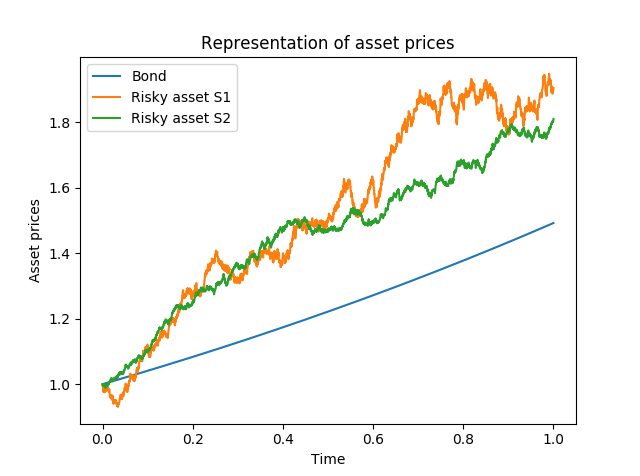
\includegraphics[width=0.7\textwidth]{images/market.png}
  \caption{Marché simulé}
\end{figure}
\frametitle{Marché}
\end{frame}

\begin{frame}
\begin{figure}[H]
  \centering
    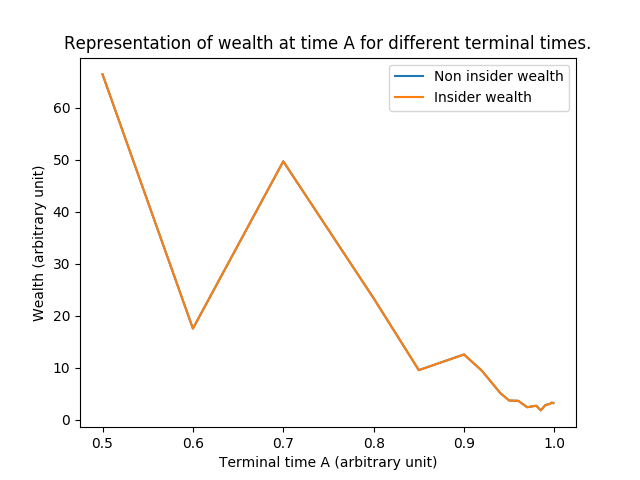
\includegraphics[width=0.7\textwidth]{images/wealths.png}
  \caption{Richesse optimale des agents en A}
\end{figure} 
\frametitle{Richesses}
\end{frame}

\begin{frame}
\begin{figure}[H]
  \centering
    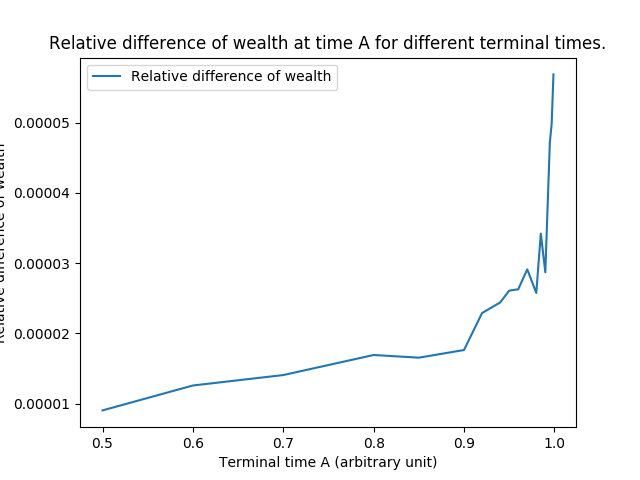
\includegraphics[width=0.7\textwidth]{images/relative_difference.png}
  \caption{Écart relatif des richesses}
\end{figure} 
\frametitle{Richesses}
\end{frame}

\section{Conclusion}
\begin{frame}
\begin{itemize}
	\item Compréhension générale du raisonnement de l'article.
	\item Implémentation informatique des formules dans un cas particulier.
\end{itemize}
\frametitle{Résumé}
\end{frame}

\begin{frame}
Approfondissement théorique : 
\begin{itemize}
	\item Cas plus réaliste : "sauts" de valeur dans le marché.
	\item Études de cas particuliers.
	\item ...
\end{itemize}
\frametitle{Perspectives du projet}
\end{frame}

\begin{frame}
\end{frame} % to enforce entries in the table of contents
\end{document}
